\documentclass[12pt]{standalone}

\usepackage{tikz}

\usetikzlibrary{decorations.markings}
\usetikzlibrary{math}

\begin{document}
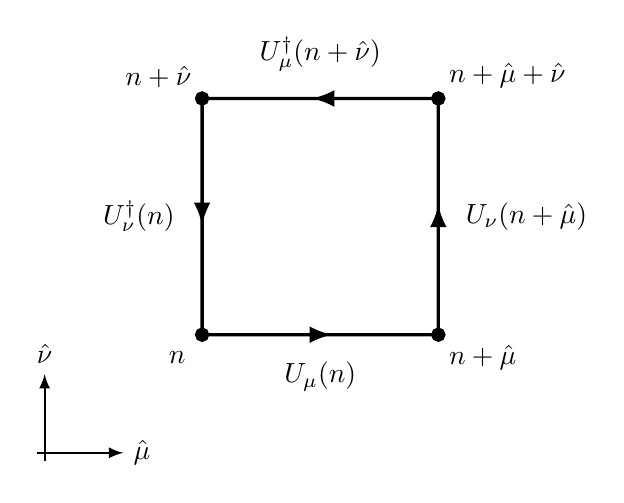
\begin{tikzpicture}

% Position settings
\tikzmath{
    \LinkLength = 3;
}

\coordinate (X0) at (0,0);
\coordinate (X1) at (\LinkLength,0);
\coordinate (X2) at (\LinkLength,\LinkLength);
\coordinate (X3) at (0,\LinkLength);

% Draws plaquette
\draw [black, 
    very thick,
    fill] 
    (X0) circle (2pt) node[below left=2.1pt] {$n$} -- (X1) circle (2pt) node [below right] {$n+\hat{\mu}$} -- (X2) circle (2pt) node [above right] {$n+\hat{\mu}+\hat{\nu}$} -- (X3) circle (2pt) node [above left] {$n+\hat{\nu}$}-- (X0);

% Draws axis
\draw [black, thick, -latex] (-2.1,-1.5) -- (-1,-1.5) node [right] {$\hat{\mu}$};
\draw [black, thick, -latex] (-2,-1.6) -- (-2,-0.5) node [above] {$\hat{\nu}$};

% Write out links
\draw [black, very thick, fill,
    decoration={markings, mark=at position 1 with {\arrow[black,scale=1.25,xshift=3.33333pt]{latex}}},
    postaction={decorate}] 
    (0.5*\LinkLength,0) node [below=6pt] {$U_\mu(n)$};
\draw [black, very thick, fill,
    decoration={markings, mark=at position 1 with {\arrow[black,scale=1.25,rotate=90,xshift=3.33333pt]{latex}}},
    postaction={decorate}] 
    (\LinkLength,0.5*\LinkLength) node [right=6pt] {$U_\nu(n+\hat{\mu})$};
\draw [black, very thick, fill,
    decoration={markings, mark=at position 1 with {\arrow[black,scale=1.25,rotate=180,xshift=2.33333pt]{latex}}},
    postaction={decorate}]
    (0.5*\LinkLength,\LinkLength) node [above=6pt] {$U^\dagger_\mu(n+\hat{\nu})$};
\draw [black, very thick, fill,
    decoration={markings, mark=at position 1 with {\arrow[black,scale=1.25,rotate=270,xshift=2.33333pt]{latex}}},
    postaction={decorate}]
    (0,0.5*\LinkLength) node [left=6pt] {$U^\dagger_\nu(n)$};


\end{tikzpicture}
\end{document}
